%% LyX 2.1.3 created this file.  For more info, see http://www.lyx.org/.
%% Do not edit unless you really know what you are doing.
\documentclass[english]{article}
\usepackage[latin9]{inputenc}
\usepackage[a4paper]{geometry}
\geometry{verbose,tmargin=1in,bmargin=1in,lmargin=0.5in,rmargin=0.5in}
\usepackage{fancyhdr}
\pagestyle{fancy}
\setlength{\parskip}{\smallskipamount}
\setlength{\parindent}{0pt}
\usepackage{babel}
\usepackage{units}
\usepackage{amsmath}
\usepackage{amssymb}
\usepackage{graphicx}
\usepackage[unicode=true,
 bookmarks=true,bookmarksnumbered=false,bookmarksopen=false,
 breaklinks=false,pdfborder={0 0 0},backref=false,colorlinks=false]
 {hyperref}
\hypersetup{pdftitle={Trigonometry Cram Sheet},
 pdfauthor={All Too Technical}}

\makeatletter

%%%%%%%%%%%%%%%%%%%%%%%%%%%%%% LyX specific LaTeX commands.
%% Because html converters don't know tabularnewline
\providecommand{\tabularnewline}{\\}

%%%%%%%%%%%%%%%%%%%%%%%%%%%%%% Textclass specific LaTeX commands.
\newenvironment{lyxlist}[1]
{\begin{list}{}
{\settowidth{\labelwidth}{#1}
 \setlength{\leftmargin}{\labelwidth}
 \addtolength{\leftmargin}{\labelsep}
 \renewcommand{\makelabel}[1]{##1\hfil}}}
{\end{list}}

%%%%%%%%%%%%%%%%%%%%%%%%%%%%%% User specified LaTeX commands.
\usepackage{pgf,tikz}
\usepackage{mathrsfs}
\usetikzlibrary{arrows}
\usepackage{multicol}
\usepackage{array}
\usepackage{pgfplots}
\usepgfplotslibrary{polar}
\usepgflibrary{shapes.geometric}
\usetikzlibrary{calc}
\pgfplotsset{my style polar/.append style={xticklabels={,, $\frac{\pi}{6}$, $\frac{\pi}{3}$, $\frac{\pi}{2}$, $\frac{2\pi}{3}$, $\frac{5\pi}{6}$, $\pi$, $\frac{7\pi}{6}$, $\frac{4\pi}{3}$, $\frac{3\pi}{2}$, $\frac{5\pi}{3}$,$\frac{11\pi}{6}$,}, thick }}

\makeatother

\begin{document}

\lhead{\textsf{\textbf{Trigonometry Cram Sheet}}}


\rhead{\textsf{\href{http://www.alltootechnical.tk}{alltootechnical.tk}}}


\title{\textsf{\textbf{Trigonometry Cram Sheet}}}


\date{\textsf{\today{}}}

\maketitle
\begin{multicols*}{2}

\tableofcontents{}

\end{multicols*}\newpage{}

\begin{multicols}{2}


\section{Definition}

Triangle $ABC$ has a right angle at $C$ and sides of length $a$,
$b$, $c$. The trigonometric functions of angle $A$ are defined
as follows:
\begin{enumerate}
\item ${\displaystyle \sin A=\frac{a}{c}=\frac{\mathrm{opposite}}{\mathrm{hypotenuse}}}$
\item ${\displaystyle \cos A=\frac{b}{c}=\frac{\mathrm{adjacent}}{\mathrm{hypotenuse}}}$
\item ${\displaystyle \tan A=\frac{a}{b}=\frac{\mathrm{opposite}}{\mathrm{adjacent}}}$
\item ${\displaystyle \csc A=\frac{c}{a}=\frac{\mathrm{hypotenuse}}{\mathrm{opposite}}}$
\item ${\displaystyle \sec A=\frac{c}{b}=\frac{\mathrm{hypotenuse}}{\mathrm{adjacent}}}$
\item ${\displaystyle \cot A=\frac{b}{a}=\frac{\mathrm{adjacent}}{\mathrm{opposite}}}$
\end{enumerate}

\subsection{Extensions to Angles $>90^{\circ}$}

A point $P$ in the Cartesian plane has coordinates $\left(x,y\right)$,
where $x$ is considered as positive along $OX$ and negative along
$OX'$, while $y$ is considered as positive along $OY'$ and negative
along $OY$. The distance from origin $O$ to point $P$ is positive
and denoted by $r=\sqrt{x^{2}+y^{2}}$. The angle $A$ described \emph{counterclockwise}
from $OX$ is considered \emph{positive}. If it is described \emph{clockwise}
from $OX$ it is considered \emph{negative}.

For an angle $A$ in any quadrant, the trigonometric functions of
$A$ are defined as follows:
\begin{enumerate}
\item ${\displaystyle \sin A=\frac{y}{r}}$
\item ${\displaystyle \cos A=\frac{x}{r}}$
\item ${\displaystyle \tan A=\frac{y}{x}}$
\item ${\displaystyle \csc A=\frac{r}{y}}$
\item ${\displaystyle \sec A=\frac{r}{x}}$
\item ${\displaystyle \cot A=\frac{x}{y}}$
\end{enumerate}

\subsection{The Unit Circle}

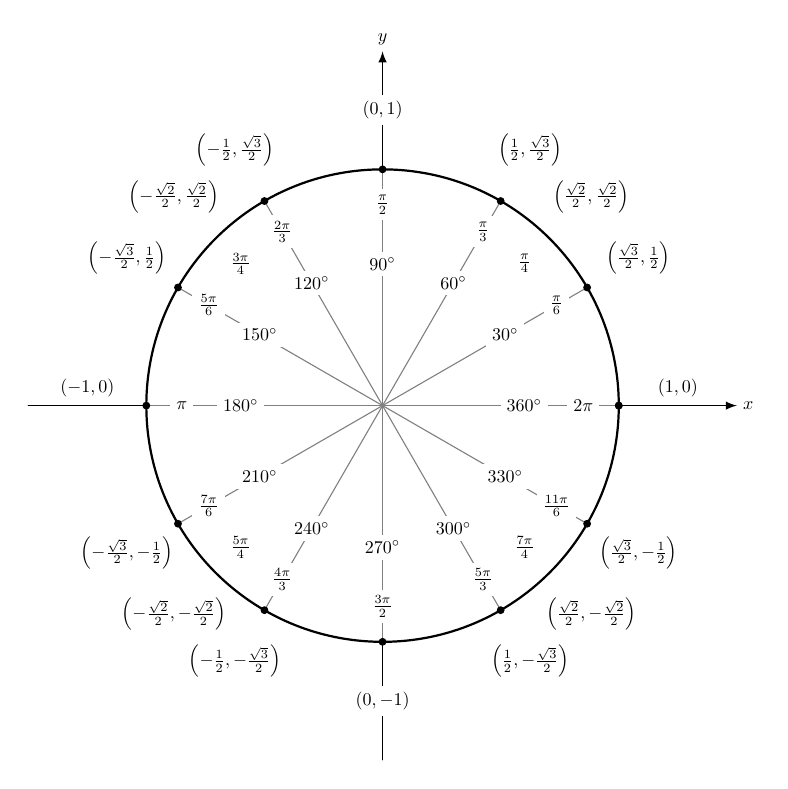
\begin{tikzpicture}[scale=3,cap=round,>=latex,every node/.style={scale=0.65}]
        % draw the coordinates
        \draw[->] (-1.5cm,0cm) -- (1.5cm,0cm) node[right,fill=white] {$x$};
        \draw[->] (0cm,-1.5cm) -- (0cm,1.5cm) node[above,fill=white] {$y$};

        % draw the unit circle
        \draw[thick] (0cm,0cm) circle(1cm);

        \foreach \x in {0,30,...,360} {
                % lines from center to point
                \draw[gray] (0cm,0cm) -- (\x:1cm);
                % dots at each point
                \filldraw[black] (\x:1cm) circle(0.4pt);
                % draw each angle in degrees
                \draw (\x:0.6cm) node[fill=white] {$\x^\circ$};
        }

        % draw each angle in radians
        \foreach \x/\xtext in {
            30/\frac{\pi}{6},
            45/\frac{\pi}{4},
            60/\frac{\pi}{3},
            90/\frac{\pi}{2},
            120/\frac{2\pi}{3},
            135/\frac{3\pi}{4},
            150/\frac{5\pi}{6},
            180/\pi,
            210/\frac{7\pi}{6},
            225/\frac{5\pi}{4},
            240/\frac{4\pi}{3},
            270/\frac{3\pi}{2},
            300/\frac{5\pi}{3},
            315/\frac{7\pi}{4},
            330/\frac{11\pi}{6},
            360/2\pi}
                \draw (\x:0.85cm) node[fill=white] {$\xtext$};

        \foreach \x/\xtext/\y in {
            % the coordinates for the first quadrant
            30/\frac{\sqrt{3}}{2}/\frac{1}{2},
            45/\frac{\sqrt{2}}{2}/\frac{\sqrt{2}}{2},
            60/\frac{1}{2}/\frac{\sqrt{3}}{2},
            % the coordinates for the second quadrant
            150/-\frac{\sqrt{3}}{2}/\frac{1}{2},
            135/-\frac{\sqrt{2}}{2}/\frac{\sqrt{2}}{2},
            120/-\frac{1}{2}/\frac{\sqrt{3}}{2},
            % the coordinates for the third quadrant
            210/-\frac{\sqrt{3}}{2}/-\frac{1}{2},
            225/-\frac{\sqrt{2}}{2}/-\frac{\sqrt{2}}{2},
            240/-\frac{1}{2}/-\frac{\sqrt{3}}{2},
            % the coordinates for the fourth quadrant
            330/\frac{\sqrt{3}}{2}/-\frac{1}{2},
            315/\frac{\sqrt{2}}{2}/-\frac{\sqrt{2}}{2},
            300/\frac{1}{2}/-\frac{\sqrt{3}}{2}}
                \draw (\x:1.25cm) node[fill=white] {$\left(\xtext,\y\right)$};

        % draw the horizontal and vertical coordinates
        % the placement is better this way
        \draw (-1.25cm,0cm) node[above=1pt] {$(-1,0)$}
              (1.25cm,0cm)  node[above=1pt] {$(1,0)$}
              (0cm,-1.25cm) node[fill=white] {$(0,-1)$}
              (0cm,1.25cm)  node[fill=white] {$(0,1)$};
    \end{tikzpicture}


\subsection{Degrees and Radians}

A \emph{radian} is that angle $\theta$ subtended at center $O$ of
a circle by an arc $MN$ equal to the radius $r$. Since $\unit[2\pi]{radians}=360\textdegree$
we have:
\begin{lyxlist}{00.00.0000}
\item [{$\unit[1]{radian}=180\textdegree/\pi=57.29577951308232\dots\textdegree$}]~
\item [{$1\textdegree=\unit[\pi/180]{radians}=\unit[0.017453292519943\dots]{radians}$}]~
\end{lyxlist}

\subsection{Signs and Variations}

\begin{tabular}{|c|c|c|c|}
\hline 
Quadrant & $\sin A$ & $\cos A$ & $\tan A$\tabularnewline
\hline 
\hline 
I & $\begin{array}{c}
+\\
\left(0,1\right)
\end{array}$ & $\begin{array}{c}
+\\
\left(1,0\right)
\end{array}$ & $\begin{array}{c}
+\\
\left(0,\infty\right)
\end{array}$\tabularnewline
\hline 
II & $\begin{array}{c}
+\\
\left(1,0\right)
\end{array}$ & $\begin{array}{c}
-\\
\left(0,-1\right)
\end{array}$ & $\begin{array}{c}
-\\
\left(-\infty,0\right)
\end{array}$\tabularnewline
\hline 
III & $\begin{array}{c}
-\\
\left(0,-1\right)
\end{array}$ & $\begin{array}{c}
-\\
\left(-1,0\right)
\end{array}$ & $\begin{array}{c}
+\\
\left(0,\infty\right)
\end{array}$\tabularnewline
\hline 
IV & $\begin{array}{c}
-\\
\left(-1,0\right)
\end{array}$ & $\begin{array}{c}
+\\
\left(0,1\right)
\end{array}$ & $\begin{array}{c}
-\\
\left(-\infty,0\right)
\end{array}$\tabularnewline
\hline 
\end{tabular}

\begin{tabular}{|c|c|c|c|}
\hline 
Quadrant & $\cot A$ & $\sec A$ & $\csc A$\tabularnewline
\hline 
\hline 
I & $\begin{array}{c}
+\\
\left(\infty,0\right)
\end{array}$ & $\begin{array}{c}
+\\
\left(1,\infty\right)
\end{array}$ & $\begin{array}{c}
+\\
\left(\infty,1\right)
\end{array}$\tabularnewline
\hline 
II & $\begin{array}{c}
-\\
\left(0,-\infty\right)
\end{array}$ & $\begin{array}{c}
-\\
\left(\infty,-1\right)
\end{array}$ & $\begin{array}{c}
+\\
\left(1,\infty\right)
\end{array}$\tabularnewline
\hline 
III & $\begin{array}{c}
+\\
\left(\infty,0\right)
\end{array}$ & $\begin{array}{c}
-\\
\left(-1,\infty\right)
\end{array}$ & $\begin{array}{c}
-\\
\left(\infty,-1\right)
\end{array}$\tabularnewline
\hline 
IV & $\begin{array}{c}
-\\
\left(0,-\infty\right)
\end{array}$ & $\begin{array}{c}
+\\
\left(\infty,1\right)
\end{array}$ & $\begin{array}{c}
-\\
\left(-1,\infty\right)
\end{array}$\tabularnewline
\hline 
\end{tabular}

\end{multicols}

\newpage{}

\begin{multicols}{2}


\section{Properties and General Forms}


\subsection{Properties}


\subsubsection{$\sin x$}
\begin{description}
\item [{Domain:}] $\left\{ x|x\in\mathbb{R}\right\} $ or $\left(-\infty,+\infty\right)$
\item [{Range:}] $\left\{ y|-1\le y\le1\right\} $ or $\left[-1,1\right]$
\item [{Period:}] $2\pi$
\item [{VA:}] none
\item [{$x$-intercepts:}] $k\pi$ where $k\in\mathbb{Z}$
\item [{Parity:}] odd
\end{description}

\subsubsection{$\cos x$}
\begin{description}
\item [{Domain:}] $\left\{ x|x\in\mathbb{R}\right\} $ or $\left(-\infty,+\infty\right)$
\item [{Range:}] $\left\{ y|-1\le y\le1\right\} $ or $\left[-1,1\right]$
\item [{Period:}] $2\pi$
\item [{VA:}] none
\item [{$x$-intercepts:}] $\frac{\pi}{2}+k\pi$ where $k\in\mathbb{Z}$
\item [{Parity:}] even
\end{description}

\subsubsection{$\tan x$}
\begin{description}
\item [{Domain:}] $\left\{ x|x\ne\frac{\pi}{2}+k\pi,k\in\mathbb{Z}\right\} $
or $\bigcup_{k\in\mathbb{Z}}\left(\frac{\left(k-1\right)\pi}{2},\frac{\left(k+1\right)\pi}{2}\right)$
\item [{Range:}] $\left\{ y|y\in\mathbb{R}\right\} $ or $\left(-\infty,+\infty\right)$
\item [{Period:}] $\pi$
\item [{VA:}] $x=\frac{\pi}{2}+k\pi$ where $k\in\mathbb{Z}$
\item [{$x$-intercepts:}] $k\pi$ where $k\in\mathbb{Z}$
\item [{Parity:}] odd
\end{description}

\subsubsection{$\csc x$}
\begin{description}
\item [{Domain:}] $\left\{ x|x\ne k\pi,k\in\mathbb{Z}\right\} $or $\bigcup_{k\in\mathbb{Z}}\left(k\pi,\left(k+1\right)\pi\right)$
\item [{Range:}] $\left\{ y|y\le1\cup y\ge1\right\} $ or $\left(-\infty,-1\right]\cup\left[1,+\infty\right)$
\item [{Period:}] $2\pi$
\item [{VA:}] $x=k\pi$ where $k\in\mathbb{Z}$
\item [{$x$-intercepts:}] none
\item [{Parity:}] odd
\end{description}

\subsubsection{$\sec x$}
\begin{description}
\item [{Domain:}] $\left\{ x|x\ne\frac{\pi}{2}+k\pi,k\in\mathbb{Z}\right\} $
or $\bigcup_{k\in\mathbb{Z}}\left(\frac{\left(k-1\right)\pi}{2},\frac{\left(k+1\right)\pi}{2}\right)$
\item [{Range:}] $\left\{ y|y\le1\cup y\ge1\right\} $ or $\left(-\infty,-1\right]\cup\left[1,+\infty\right)$
\item [{Period:}] $2\pi$
\item [{VA:}] $x=\frac{\pi}{2}+k\pi$ where $k\in\mathbb{Z}$
\item [{$x$-intercepts:}] none
\item [{Parity:}] even
\end{description}

\subsubsection{$\cot x$}
\begin{description}
\item [{Domain:}] $\left\{ x|x\ne k\pi,k\in\mathbb{Z}\right\} $ or $\bigcup_{k\in\mathbb{Z}}\left(k\pi,\left(k+1\right)\pi\right)$
\item [{Range:}] $\left\{ y|y\in\mathbb{R}\right\} $ or $\left(-\infty,+\infty\right)$
\item [{Period:}] $\pi$
\item [{VA:}] $x=k\pi$ where $k\in\mathbb{Z}$
\item [{$x$-intercepts:}] $\frac{\pi}{2}+k\pi$ where $k\in\mathbb{Z}$
\item [{Parity:}] odd
\end{description}
\end{multicols}


\subsection{General Forms of Trigonometric Functions}

Given some trigonometric function $f\left(x\right)$, its general
form is represented as $y=Af\left(B\left(x-C\right)\right)+D$, where
its amplitude is $\left|A\right|$, its period is $\frac{2\pi}{\left|B\right|}$
or $\frac{\pi}{\left|B\right|}$ (for tangent and cotangent), its
phase shift is $C$, and its vertical translation is $D$ units upward
(if $D>0$) or $D$ units downward (if $D<0$). The maximum and minimum
value for $\sin x$ and $\cos x$ is $A+D$ and $-A+D$ respectively. 

\vfill{}


\renewcommand{\arraystretch}{1.5}

\begin{tabular}{|c|c|c|c|}
\hline 
amplitude & period & phase shift & vertical translation\tabularnewline
\hline 
\definecolor{yqyqyq}{rgb}{0.5019607843137255,0.5019607843137255,0.5019607843137255} \begin{tikzpicture}[line cap=round,line join=round,>=triangle 45,x=0.75cm,y=0.75cm] \draw[->,color=black] (-1,0) -- (4,0); \foreach \x in {-1,1,2,3} \draw[shift={(\x,0)},color=black] (0pt,2pt) -- (0pt,-2pt) node[below] {\footnotesize $\x$}; \draw[->,color=black] (0,-2) -- (0,2); \foreach \y in {-2,-1,1} \draw[shift={(0,\y)},color=black] (2pt,0pt) -- (-2pt,0pt) node[left] {\footnotesize $\y$}; \draw[color=black] (0pt,-10pt) node[right] {\footnotesize $0$}; \clip(-1,-2) rectangle (4,2); \draw[line width=1.2pt,dash pattern=on 1pt off 1pt,color=yqyqyq,smooth,samples=100,domain=-1.0:4.0] plot(\x,{sin(((\x))*180/pi)}); \draw[line width=1.6pt,smooth,samples=100,domain=-1.0:4.0] plot(\x,{1.75*sin(((\x))*180/pi)}); \begin{scriptsize} \draw[color=yqyqyq] (-5.64,0.42) node {$f$}; \draw[color=black] (-5.64,-0.98) node {$a$}; \end{scriptsize} \end{tikzpicture}  & \definecolor{yqyqyq}{rgb}{0.5019607843137255,0.5019607843137255,0.5019607843137255} \begin{tikzpicture}[line cap=round,line join=round,>=triangle 45,x=0.75cm,y=0.75cm] \draw[->,color=black] (-1,0) -- (4,0); \foreach \x in {-1,1,2,3} \draw[shift={(\x,0)},color=black] (0pt,2pt) -- (0pt,-2pt) node[below] {\footnotesize $\x$}; \draw[->,color=black] (0,-2) -- (0,2); \foreach \y in {-2,-1,1} \draw[shift={(0,\y)},color=black] (2pt,0pt) -- (-2pt,0pt) node[left] {\footnotesize $\y$}; \draw[color=black] (0pt,-10pt) node[right] {\footnotesize $0$}; \clip(-1,-2) rectangle (4,2); \draw[line width=1.2pt,dash pattern=on 1pt off 1pt,color=yqyqyq,smooth,samples=100,domain=-1.0:4.0] plot(\x,{sin(((\x))*180/pi)}); \draw[line width=1.6pt,smooth,samples=100,domain=-1.0:4.0] plot(\x,{sin((2.0*(\x))*180/pi)}); \begin{scriptsize} \draw[color=yqyqyq] (-5.64,0.42) node {$f$}; \draw[color=black] (-5.64,-0.98) node {$a$}; \end{scriptsize} \end{tikzpicture} & \definecolor{yqyqyq}{rgb}{0.5019607843137255,0.5019607843137255,0.5019607843137255} \begin{tikzpicture}[line cap=round,line join=round,>=triangle 45,x=0.75cm,y=0.75cm] \draw[->,color=black] (-1,0) -- (4,0); \foreach \x in {-1,1,2,3} \draw[shift={(\x,0)},color=black] (0pt,2pt) -- (0pt,-2pt) node[below] {\footnotesize $\x$}; \draw[->,color=black] (0,-2) -- (0,2); \foreach \y in {-2,-1,1} \draw[shift={(0,\y)},color=black] (2pt,0pt) -- (-2pt,0pt) node[left] {\footnotesize $\y$}; \draw[color=black] (0pt,-10pt) node[right] {\footnotesize $0$}; \clip(-1,-2) rectangle (4,2); \draw[line width=1.2pt,dash pattern=on 1pt off 1pt,color=yqyqyq,smooth,samples=100,domain=-1.0:4.0] plot(\x,{sin(((\x))*180/pi)}); \draw[line width=1.6pt,smooth,samples=100,domain=-1.0:4.0] plot(\x,{sin(((\x)-3.1415926535/2.0)*180/pi)}); \begin{scriptsize} \draw[color=yqyqyq] (-5.64,0.42) node {$f$}; \draw[color=black] (-5.64,-0.98) node {$a$}; \end{scriptsize} \end{tikzpicture} & \definecolor{yqyqyq}{rgb}{0.5019607843137255,0.5019607843137255,0.5019607843137255} \begin{tikzpicture}[line cap=round,line join=round,>=triangle 45,x=0.75cm,y=0.75cm] \draw[->,color=black] (-1,0) -- (4,0); \foreach \x in {-1,1,2,3} \draw[shift={(\x,0)},color=black] (0pt,2pt) -- (0pt,-2pt) node[below] {\footnotesize $\x$}; \draw[->,color=black] (0,-2) -- (0,2); \foreach \y in {-2,-1,1} \draw[shift={(0,\y)},color=black] (2pt,0pt) -- (-2pt,0pt) node[left] {\footnotesize $\y$}; \draw[color=black] (0pt,-10pt) node[right] {\footnotesize $0$}; \clip(-1,-2) rectangle (4,2); \draw[line width=1.2pt,dash pattern=on 1pt off 1pt,color=yqyqyq,smooth,samples=100,domain=-1.0:4.0] plot(\x,{sin(((\x))*180/pi)}); \draw[line width=1.6pt,smooth,samples=100,domain=-1.0:4.0] plot(\x,{sin(((\x))*180/pi)-1}); \begin{scriptsize} \draw[color=yqyqyq] (-5.64,0.42) node {$f$}; \draw[color=black] (-5.64,-0.98) node {$a$}; \end{scriptsize} \end{tikzpicture} \tabularnewline
\hline 
\end{tabular}

\newpage{}

\begin{multicols}{2}


\section{Identities}


\subsection{Basic Identities}


\subsubsection{Reciprocal Identities}
\begin{lyxlist}{00.00.0000}
\item [{${\displaystyle \csc\theta=\frac{1}{\sin\theta}}$;$\quad{\displaystyle \sin\theta=\frac{1}{\csc\theta}}$}]~
\item [{${\displaystyle \sec\theta=\frac{1}{\cos\theta}}$;$\quad{\displaystyle \cos\theta=\frac{1}{\sec\theta}}$}]~
\item [{${\displaystyle \cot\theta=\frac{1}{\tan\theta}}$;$\quad{\displaystyle \tan\theta=\frac{1}{\cot\theta}}$}]~
\item [{${\displaystyle \sin\theta\csc\theta=\cos\theta\sec\theta=\tan\theta\cot\theta=1}$}]~
\end{lyxlist}

\subsubsection{Ratio Identities}
\begin{lyxlist}{00.00.0000}
\item [{${\displaystyle \tan\theta=\frac{\sin\theta}{\cos\theta}}$;$\quad{\displaystyle \cos\theta=\frac{\sin\theta}{\tan\theta}}$;$\quad{\displaystyle \sin\theta=\cos\theta\tan\theta}$}]~
\item [{${\displaystyle \cot\theta=\frac{\cos\theta}{\sin\theta}}$;$\quad{\displaystyle \sin\theta=\frac{\cos\theta}{\cot\theta}}$;$\quad\cos\theta=\sin\theta\cot\theta$}]~
\end{lyxlist}

\subsubsection{Pythagorean Identities}
\begin{lyxlist}{00.00.0000}
\item [{${\displaystyle \sin^{2}\theta+\cos^{2}\theta=1}$;}] ${\displaystyle \sin^{2}\theta=1-\cos^{2}\theta}$;
${\displaystyle \cos^{2}\theta=1-\sin^{2}\theta}$
\item [{${\displaystyle \tan^{2}\theta+1=\sec^{2}\theta}$;}] ${\displaystyle \tan^{2}\theta=\sec^{2}\theta-1}$;
${\displaystyle \sec^{2}\theta-\tan^{2}\theta=1}$
\item [{${\displaystyle \cot^{2}\theta+1=\csc^{2}\theta}$;}] ${\displaystyle \cot^{2}\theta=\csc^{2}\theta-1}$;
${\displaystyle \csc^{2}\theta-\cot^{2}\theta=1}$
\end{lyxlist}

\subsubsection{Co-function Identities}
\begin{lyxlist}{00.00.0000}
\item [{${\displaystyle \sin\left(\frac{\pi}{2}-\theta\right)=\cos\theta}$}]~
\item [{${\displaystyle \cos\left(\frac{\pi}{2}-\theta\right)=\sin\theta}$}]~
\item [{${\displaystyle \tan\left(\frac{\pi}{2}-\theta\right)=\cot\theta}$}]~
\item [{${\displaystyle \csc\left(\frac{\pi}{2}-\theta\right)=\sec\theta}$}]~
\item [{${\displaystyle \sec\left(\frac{\pi}{2}-\theta\right)=\csc\theta}$}]~
\item [{${\displaystyle \cot\left(\frac{\pi}{2}-\theta\right)=\tan\theta}$}]~
\end{lyxlist}

\subsubsection{Parity Identities}
\begin{lyxlist}{00.00.0000}
\item [{$\sin\left(-A\right)=-\sin A$}]~
\item [{$\cos\left(-A\right)=\cos A$}]~
\item [{$\tan\left(-A\right)=-\tan A$}]~
\item [{$\csc\left(-A\right)=-\csc A$}]~
\item [{$\sec\left(-A\right)=\sec A$}]~
\item [{$\cot\left(-A\right)=-\cot A$}]~
\end{lyxlist}

\subsection{Sum and Difference}
\begin{lyxlist}{00.00.0000}
\item [{${\displaystyle \sin\left(\alpha\pm\beta\right)=\sin\alpha\cos\beta\pm\cos\alpha\sin\beta}$}]~
\item [{${\displaystyle \cos\left(\alpha\pm\beta\right)=\cos\alpha\cos\beta\mp\sin\alpha\sin\beta}$}]~
\item [{${\displaystyle \tan\left(\alpha\pm\beta\right)=\frac{\tan\alpha\pm\tan\beta}{1\mp\tan\alpha\tan\beta}}$}]~
\item [{${\displaystyle \cot\left(\alpha\pm\beta\right)=\frac{\cot\alpha\cot\beta\mp1}{\cot\beta\pm\cot\alpha}}$}]~
\end{lyxlist}

\subsection{Double Angle}
\begin{lyxlist}{00.00.0000}
\item [{${\displaystyle \sin2\alpha=2\sin\alpha\cos\alpha}$}]~
\item [{$\cos2\alpha=\cos^{2}\alpha-\sin^{2}\alpha=1-2\sin^{2}\alpha=2\cos^{2}\alpha-1$}]~
\item [{${\displaystyle \tan2\alpha=\frac{2\tan\alpha}{1-\tan^{2}\alpha}}$}]~
\end{lyxlist}

\subsection{Half Angle}

Let $\mathcal{Q}_{n}$, where $n\in\left\{ 1,2,3,4\right\} $, denote
the set of all angles within the $n$\textsuperscript{th} quadrant
of the Cartesian plane.
\begin{lyxlist}{00.00.0000}
\item [{${\displaystyle \sin\frac{\alpha}{2}=\begin{cases}
\sqrt{\frac{1-\cos\alpha}{2}} & \text{if }\frac{\alpha}{2}\in\left(\mathcal{Q}_{1}\cup\mathcal{Q}_{2}\right)\\
-\sqrt{\frac{1-\cos\alpha}{2}} & \text{if }\frac{\alpha}{2}\in\left(\mathcal{Q}_{3}\cup\mathcal{Q}_{4}\right)
\end{cases}}$}]~
\item [{${\displaystyle \cos\frac{\alpha}{2}=\begin{cases}
\sqrt{\frac{1+\cos\alpha}{2}} & \text{if }\frac{\alpha}{2}\in\left(\mathcal{Q}_{1}\cup\mathcal{Q}_{4}\right)\\
-\sqrt{\frac{1+\cos\alpha}{2}} & \text{if }\frac{\alpha}{2}\in\left(\mathcal{Q}_{2}\cup\mathcal{Q}_{3}\right)
\end{cases}}$}]~
\item [{${\displaystyle \tan\frac{\alpha}{2}=\frac{\sin\alpha}{1+\cos\alpha}=\frac{1-\cos\alpha}{\sin\alpha}=\csc\alpha-\cot\alpha}$}]~
\end{lyxlist}

\subsection{Multiple Angle}
\begin{lyxlist}{00.00.0000}
\item [{$\sin3\alpha=3\sin\alpha-4\sin^{3}\alpha$}]~
\item [{$\cos3\alpha=4\cos^{3}\alpha-3\cos\alpha$}]~
\item [{${\displaystyle \tan3\alpha=\frac{3\tan\alpha-\tan^{3}\alpha}{1-3\tan^{2}\alpha}}$}]~
\item [{${\displaystyle \sin4\alpha=4\sin\alpha\cos\alpha-8\sin^{3}\alpha\cos\alpha}$}]~
\item [{${\displaystyle \cos4\alpha=8\cos^{4}\alpha-8\cos^{2}\alpha+1}$}]~
\item [{${\displaystyle \tan4\alpha=\frac{4\tan\alpha-4\tan^{3}\alpha}{1-6\tan^{2}\alpha+\tan^{4}\alpha}}$}]~
\item [{${\displaystyle \sin\left(n\alpha\right)=\sum_{i=0}^{n}\binom{n}{i}\cos^{i}\alpha\sin^{n-i}\alpha\sin\left(\frac{\left(n-i\right)\pi}{2}\right)}$}]~
\item [{${\displaystyle \cos\left(n\alpha\right)=\sum_{i=0}^{n}\binom{n}{i}\cos^{i}\alpha\sin^{n-i}\alpha\cos\left(\frac{\left(n-i\right)\pi}{2}\right)}$}]~
\end{lyxlist}

\subsection{Power Reduction}
\begin{lyxlist}{00.00.0000}
\item [{${\displaystyle \sin^{2}\theta=\frac{1-\cos2\theta}{2}}$}]~
\item [{${\displaystyle \cos^{2}\theta=\frac{1+\cos2\theta}{2}}$}]~
\item [{${\displaystyle \tan^{2}\theta=\frac{1-\cos2\theta}{1+\cos2\theta}}$}]~
\item [{${\displaystyle \sin^{3}\theta=\frac{3\sin\theta-\sin3\theta}{4}}$}]~
\item [{${\displaystyle \cos^{3}\theta=\frac{3\cos\theta+\cos3\theta}{4}}$}]~
\item [{${\displaystyle \sin^{4}\theta=\frac{3-4\cos2\theta+\cos4\theta}{8}}$}]~
\item [{${\displaystyle \cos^{4}\theta=\frac{3+4\cos2\theta+\cos4\theta}{8}}$}]~
\item [{${\displaystyle \sin^{5}\theta=\frac{10\sin\theta-5\sin3\theta+\sin5\theta}{16}}$}]~
\item [{${\displaystyle \cos^{5}\theta=\frac{10\cos\theta+5\cos3\theta+\cos5\theta}{16}}$}]~
\end{lyxlist}

\subsection{Product to Sum}
\begin{lyxlist}{00.00.0000}
\item [{${\displaystyle \sin\alpha\cos\beta=\frac{1}{2}\left[\sin\left(\alpha+\beta\right)+\sin\left(\alpha-\beta\right)\right]}$}]~
\item [{${\displaystyle \cos\alpha\sin\beta=\frac{1}{2}\left[\sin\left(\alpha+\beta\right)-\sin\left(\alpha-\beta\right)\right]}$}]~
\item [{${\displaystyle \cos\alpha\cos\beta=\frac{1}{2}\left[\cos\left(\alpha+\beta\right)+\cos\left(\alpha-\beta\right)\right]}$}]~
\item [{${\displaystyle \sin\alpha\sin\beta=\frac{1}{2}\left[\cos\left(\alpha+\beta\right)-\cos\left(\alpha-\beta\right)\right]}$}]~
\end{lyxlist}

\subsection{Sum to Product}
\begin{lyxlist}{00.00.0000}
\item [{${\displaystyle \sin\theta\pm\sin\varphi=2\sin\frac{\theta\pm\varphi}{2}\cos\frac{\theta\mp\varphi}{2}}$}]~
\item [{${\displaystyle \cos\theta+\cos\varphi=2\cos\frac{\theta+\varphi}{2}\cos\frac{\theta-\varphi}{2}}$}]~
\item [{${\displaystyle \cos\theta-\cos\varphi=-2\sin\frac{\theta+\varphi}{2}\sin\frac{\theta-\varphi}{2}}$}]~
\end{lyxlist}

\subsection{Linear Combinations}

For some purposes it is important to know that any linear combination
of sine waves of the same period or frequency but different phase
shifts is also a sine wave with the same period or frequency, but
a different phase shift.


\subsubsection*{Definition}

The two-argument form of the arctangent function, denoted by $\tan^{-1}\left(y,x\right)$
gathers information on the signs of the inputs in order to return
the appropriate quadrant of the computed angle. Thus, it is defined
as:

$\tan^{-1}(y,x)=\begin{cases}
\tan^{-1}\left(\frac{y}{x}\right) & \text{if }x>0,\\
\tan^{-1}\left(\frac{y}{x}\right)+\pi & \text{if }x<0\text{ and }y\ge0,\\
\tan^{-1}\left(\frac{y}{x}\right)-\pi & \text{if }x<0\text{ and }y<0,\\
+\frac{\pi}{2} & \text{if }x=0\text{ and }y>0,\\
-\frac{\pi}{2} & \text{if }x=0\text{ and }y<0,\\
\text{undefined} & \text{if }x=0\text{ and }y=0.
\end{cases}$


\subsubsection{Sine and Cosine}

In the case of a non-zero linear combination of a sine and cosine
wave (which is just a sine wave with a phase shift of $\frac{\pi}{2}$),
we have:

\noindent \begin{center}
${\displaystyle a\sin x+b\cos x=c\sin\left(x+\theta\right)}$
\par\end{center}

where $c=\pm\sqrt{a^{2}+b^{2}}$ and $\theta$ satisfies the equations
$c\cos\theta=a$ and $c\sin\theta=b$, or $\theta=\tan^{-1}\left(b,a\right)$.


\subsubsection{Arbitrary Phase Shift}

More generally, for an arbitrary phase shift, we have:

\noindent \begin{center}
${\displaystyle a\sin x+b\sin\left(x+\theta\right)=c\sin\left(x+\varphi\right)}$
\par\end{center}

where $c=\sqrt{a^{2}+b^{2}+2ab\cos\theta}$, and $\varphi$ satisfies
the equations $c\cos\varphi=a+b\cos\theta$ and $c\sin\varphi=b\sin\theta$
or $\varphi=\tan^{-1}\left(b\sin\theta,a+b\cos\theta\right)$.


\subsection{Other Related Identities}
\begin{itemize}
\item If $x+y+z=\pi$, then $\sin2x+\sin2y+\sin2z=4\sin x\sin y\sin z$.
\item \emph{Triple Tangent Identity.} If $x+y+z=\pi$, then $\tan x+\tan y+\tan z=\tan x\tan y\tan z$.
\item \emph{Triple Cotangent Identity.} If $x+y+z=\frac{\pi}{2}$, then
$\cot x+\cot y+\cot z=\cot x\cot y\cot z$.
\item \emph{Ptolemy's Theorem.} If $w+x+y+z=\pi$, then $\sin\left(w+x\right)\sin\left(x+y\right)=\sin w\sin y+\sin x\sin z$.
\item $\cot x\cot y+\cot y\cot z+\cot z\cot x=1$
\item $a\cos x+b\sin x=\sqrt{a^{2}+b^{2}}\cos\left(x-\tan^{-1}\left(b,a\right)\right)$
\item \emph{Tangent of an Average.} $\tan\left(\frac{\alpha+\beta}{2}\right)=\frac{\sin\alpha+\sin\beta}{\cos\alpha+\cos\beta}=-\frac{\cos\alpha-\cos\beta}{\sin\alpha-\sin\beta}$
\item $\tan x+\sec x=\tan\left(\frac{x}{2}+\frac{\pi}{4}\right)$
\item ${\displaystyle \sum_{i=0}^{n}\sin\left(\varphi+i\alpha\right)=\frac{\sin\frac{\left(n+1\right)\alpha}{2}\sin\left(\varphi+\frac{n\alpha}{2}\right)}{\sin\frac{\alpha}{2}}}$
\item ${\displaystyle \sum_{i=0}^{n}\cos\left(\varphi+i\alpha\right)=\frac{\sin\frac{\left(n+1\right)\alpha}{2}\cos\left(\varphi+\frac{n\alpha}{2}\right)}{\sin\frac{\alpha}{2}}}$
\item ${\displaystyle \sum_{n=1}^{\infty}\prod_{m=1}^{n}\cos\frac{m\pi}{2n+1}=1}$
\end{itemize}

\subsection{Identities without Variables}
\begin{itemize}
\item \emph{Morrie's Law.} ${\displaystyle \cos20\textdegree\cdot\cos40\textdegree\cdot\cos80\textdegree=\frac{1}{8}}$
\item ${\displaystyle \sin20\textdegree\cdot\sin40\textdegree\cdot\sin80\textdegree=\frac{\sqrt{3}}{8}}$
\item ${\displaystyle \cos24^{\circ}+\cos48^{\circ}+\cos96^{\circ}+\cos168^{\circ}=\frac{1}{2}}$
\item $\cos\frac{2\pi}{21}+\cos\left(2\cdot\frac{2\pi}{21}\right)+\cos\left(4\cdot\frac{2\pi}{21}\right)+\cos\left(5\cdot\frac{2\pi}{21}\right)+\cos\left(8\cdot\frac{2\pi}{21}\right)+\cos\left(10\cdot\frac{2\pi}{21}\right)=\frac{1}{2}$
\item ${\displaystyle \cos\frac{\pi}{5}=\cos36^{\circ}=\tfrac{1}{4}(\sqrt{5}+1)=\tfrac{1}{2}\varphi}$
\item ${\displaystyle \sin\frac{\pi}{10}=\sin18^{\circ}=\tfrac{1}{4}(\sqrt{5}-1)=\tfrac{1}{2}\varphi^{-1}}$
\item $\sin^{2}18^{\circ}+\sin^{2}30^{\circ}=\sin^{2}36^{\circ}$
\end{itemize}
\end{multicols}


\section{Graphs}

\pgfkeys{/pgfplots/Axis Style/.style={ width=13.5cm, height=5cm, axis x line=center, axis y line=middle, samples=100, ymin=-1.5, ymax=1.5, xmin=-7.0, xmax=7.0, domain=-2*pi:2*pi }}


\subsection{$y=\sin x$}

\begin{tikzpicture} \begin{axis}[ Axis Style, xtick={ -6.28318, -4.7123889, -3.14159, -1.5708, 1.5708, 3.14159, 4.7123889, 6.28318 }, xticklabels={ $-2\pi$, $-\frac{3\pi}{2}$, $-\pi$, $\frac{\pi}{2}$, $\frac{\pi}{2}$, $\pi$, $\frac{3\pi}{2}$, $2\pi$ } ] \addplot [mark=none, ultra thick, blue] {sin(deg(x))}; \end{axis} \end{tikzpicture}


\subsection{$y=\cos x$}

\begin{tikzpicture} \begin{axis}[ Axis Style, xtick={ -6.28318, -4.7123889, -3.14159, -1.5708, 1.5708, 3.14159, 4.7123889, 6.28318 }, xticklabels={ $-2\pi$, $-\frac{3\pi}{2}$, $-\pi$, $\frac{\pi}{2}$, $\frac{\pi}{2}$, $\pi$, $\frac{3\pi}{2}$, $2\pi$ } ] \addplot [mark=none, ultra thick, blue] {cos(deg(x))}; \end{axis} \end{tikzpicture}


\subsection{$y=\tan x$}

\begin{tikzpicture} \begin{axis}[ Axis Style, xtick={ -6.28318, -4.7123889, -3.14159, -1.5708, 1.5708, 3.14159, 4.7123889, 6.28318 }, xticklabels={ $-2\pi$, $-\frac{3\pi}{2}$, $-\pi$, $\frac{\pi}{2}$, $\frac{\pi}{2}$, $\pi$, $\frac{3\pi}{2}$, $2\pi$ } ] \addplot [mark=none, ultra thick, blue] {tan(deg(x))}; \end{axis} \end{tikzpicture}

\newpage{}


\section{Tables }


\subsection{Exact Values of Trigonometric Functions}

\renewcommand{\arraystretch}{2}

\noindent \begin{center}
\begin{tabular}{|c|c||c|c|c|c|c|c|}
\hline 
$A\textdegree$ & $A$ rad & $\sin A$ & $\cos A$ & $\tan A$ & $\cot A$ & $\sec A$ & $\csc A$\tabularnewline
\hline 
\hline 
$0\textdegree$ & $0$ & $0$ & $1$ & $0$ & $\infty$ & $1$ & $\infty$\tabularnewline
$15\textdegree$ & $\pi/12$ & $\frac{1}{4}\left(\sqrt{6}-\sqrt{2}\right)$ & $\frac{1}{4}\left(\sqrt{6}+\sqrt{2}\right)$ & $2-\sqrt{3}$ & $2+\sqrt{3}$ & $\sqrt{6}-\sqrt{2}$ & $\sqrt{6}+\sqrt{2}$\tabularnewline
$30\textdegree$ & $\pi/6$ & $\frac{1}{2}$ & $\frac{1}{2}\sqrt{3}$ & $\frac{1}{3}\sqrt{3}$ & $\sqrt{3}$ & $\frac{2}{3}\sqrt{3}$ & $2$\tabularnewline
$45\textdegree$ & $\pi/4$ & $\frac{1}{2}\sqrt{2}$ & $\frac{1}{2}\sqrt{2}$ & $1$ & $1$ & $\sqrt{2}$ & $\sqrt{2}$\tabularnewline
$60\textdegree$ & $\pi/3$ & $\frac{1}{2}\sqrt{3}$ & $\frac{1}{2}$ & $\sqrt{3}$ & $\frac{1}{3}\sqrt{3}$ & $2$ & $\frac{2}{3}\sqrt{3}$\tabularnewline
$75\textdegree$ & $5\pi/12$ & $\frac{1}{4}\left(\sqrt{6}+\sqrt{2}\right)$ & $\frac{1}{4}\left(\sqrt{6}-\sqrt{2}\right)$ & $2+\sqrt{3}$ & $2-\sqrt{3}$ & $\sqrt{6}+\sqrt{2}$ & $\sqrt{6}-\sqrt{2}$\tabularnewline
$90\textdegree$ & $\pi/2$ & $1$ & $0$ & $\pm\infty$ & $0$ & $\pm\infty$ & $1$\tabularnewline
$105\textdegree$ & $7\pi/12$ & $\frac{1}{4}\left(\sqrt{6}+\sqrt{2}\right)$ & $-\frac{1}{4}\left(\sqrt{6}-\sqrt{2}\right)$ & $-\left(2+\sqrt{3}\right)$ & $-\left(2-\sqrt{3}\right)$ & $-\left(\sqrt{6}+\sqrt{2}\right)$ & $\sqrt{6}-\sqrt{2}$\tabularnewline
$120\textdegree$ & $2\pi/3$ & $\frac{1}{2}\sqrt{3}$ & $\frac{1}{2}$ & $-\sqrt{3}$ & $-\frac{1}{3}\sqrt{3}$ & $-2$ & $\frac{2}{3}\sqrt{3}$\tabularnewline
$135\textdegree$ & $3\pi/4$ & $\frac{1}{2}\sqrt{2}$ & $-\frac{1}{2}\sqrt{2}$ & $-1$ & $-1$ & $-\sqrt{2}$ & $\sqrt{2}$\tabularnewline
$150\textdegree$ & $5\pi/6$ & $\frac{1}{2}$ & $-\frac{1}{2}\sqrt{3}$ & $-\frac{1}{3}\sqrt{3}$ & $-\sqrt{3}$ & $-\frac{2}{3}\sqrt{3}$ & $2$\tabularnewline
$165\textdegree$ & $11\pi/12$ & $\frac{1}{4}\left(\sqrt{6}-\sqrt{2}\right)$ & $-\frac{1}{4}\left(\sqrt{6}+\sqrt{2}\right)$ & $-\left(2-\sqrt{3}\right)$ & $-\left(2+\sqrt{3}\right)$ & $-\left(\sqrt{6}-\sqrt{2}\right)$ & $\sqrt{6}+\sqrt{2}$\tabularnewline
$180\textdegree$ & $\pi$ & $0$ & $-1$ & $0$ & $\mp\infty$ & $-1$ & $\pm\infty$\tabularnewline
$195\textdegree$ & $13\pi/12$ & $-\frac{1}{4}\left(\sqrt{6}-\sqrt{2}\right)$ & $-\frac{1}{4}\left(\sqrt{6}+\sqrt{2}\right)$ & $2-\sqrt{3}$ & $2+\sqrt{3}$ & $-\left(\sqrt{6}-\sqrt{2}\right)$ & $-\left(\sqrt{6}+\sqrt{2}\right)$\tabularnewline
$210\textdegree$ & $7\pi/6$ & $\frac{1}{2}$ & $-\frac{1}{2}\sqrt{3}$ & $\frac{1}{3}\sqrt{3}$ & $\sqrt{3}$ & $-\frac{2}{3}\sqrt{3}$ & $-2$\tabularnewline
$225\textdegree$ & $5\pi/4$ & $-\frac{1}{2}\sqrt{2}$ & $-\frac{1}{2}\sqrt{2}$ & $1$ & $1$ & $-\sqrt{2}$ & $-\sqrt{2}$\tabularnewline
$240\textdegree$ & $4\pi/3$ & $-\frac{1}{2}\sqrt{3}$ & $-\frac{1}{2}$ & $\sqrt{3}$ & $\frac{1}{3}\sqrt{3}$ & $-2$ & $-\frac{2}{3}\sqrt{3}$\tabularnewline
$255\textdegree$ & $17\pi/12$ & $-\frac{1}{4}\left(\sqrt{6}+\sqrt{2}\right)$ & $-\frac{1}{4}\left(\sqrt{6}-\sqrt{2}\right)$ & $2+\sqrt{3}$ & $2-\sqrt{3}$ & $-\left(\sqrt{6}+\sqrt{2}\right)$ & $-\left(\sqrt{6}-\sqrt{2}\right)$\tabularnewline
$270\textdegree$ & $3\pi/2$ & $-1$ & $0$ & $\pm\infty$ & $0$ & $\mp\infty$ & $-1$\tabularnewline
$285\textdegree$ & $19\pi/12$ & $-\frac{1}{4}\left(\sqrt{6}+\sqrt{2}\right)$ & $\frac{1}{4}\left(\sqrt{6}-\sqrt{2}\right)$ & $-\left(2+\sqrt{3}\right)$ & $-\left(2-\sqrt{3}\right)$ & $\sqrt{6}+\sqrt{2}$ & $-\left(\sqrt{6}-\sqrt{2}\right)$\tabularnewline
$300\textdegree$ & $5\pi/3$ & $-\frac{1}{2}\sqrt{3}$ & $\frac{1}{2}$ & $-\sqrt{3}$ & $-\frac{1}{3}\sqrt{3}$ & $2$ & $-\frac{2}{3}\sqrt{3}$\tabularnewline
$315\textdegree$ & $7\pi/4$ & $-\frac{1}{2}\sqrt{2}$ & $\frac{1}{2}\sqrt{2}$ & $-1$ & $-1$ & $\sqrt{2}$ & $-\sqrt{2}$\tabularnewline
$330\textdegree$ & $11\pi/6$ & $-\frac{1}{2}$ & $\frac{1}{2}\sqrt{3}$ & $-\frac{1}{3}\sqrt{3}$ & $-\sqrt{3}$ & $\frac{2}{3}\sqrt{3}$ & $-2$\tabularnewline
$345\textdegree$ & $23\pi/12$ & $-\frac{1}{4}\left(\sqrt{6}-\sqrt{2}\right)$ & $\frac{1}{4}\left(\sqrt{6}+\sqrt{2}\right)$ & $-\left(2+\sqrt{3}\right)$ & $-\left(2+\sqrt{3}\right)$ & $\sqrt{6}-\sqrt{2}$ & $-\left(\sqrt{6}+\sqrt{2}\right)$\tabularnewline
$360\textdegree$ & $2\pi$ & $0$ & $1$ & $0$ & $\mp\infty$ & $1$ & $\mp\infty$\tabularnewline
\hline 
\end{tabular}
\par\end{center}

\newpage{}


\subsection{Relations Between Trig Functions}

\renewcommand{\arraystretch}{2.5}

\noindent \begin{center}
\begin{tabular}{|c||c|c|c|c|c|c|}
\hline 
 & $\sin\theta=u$ & $\cos\theta=u$ & $\tan\theta=u$ & $\csc\theta=u$ & $\sec\theta=u$ & $\cot\theta=u$\tabularnewline
\hline 
\hline 
$\sin\theta$ & $u$ & $\sqrt{1-u^{2}}$ & ${\displaystyle \frac{u}{\sqrt{1+u^{2}}}}$ & ${\displaystyle \frac{1}{u}}$ & ${\displaystyle \frac{\sqrt{u^{2}-1}}{u}}$ & ${\displaystyle \frac{1}{\sqrt{1+u^{2}}}}$\tabularnewline
$\cos\theta$ & $\sqrt{1-u^{2}}$ & $u$ & ${\displaystyle \frac{1}{\sqrt{1+u^{2}}}}$ & ${\displaystyle \frac{\sqrt{u^{2}-1}}{u}}$ & ${\displaystyle \frac{1}{u}}$ & ${\displaystyle \frac{u}{\sqrt{1+u^{2}}}}$\tabularnewline
$\tan\theta$ & ${\displaystyle \frac{u}{\sqrt{1-u^{2}}}}$ & ${\displaystyle \frac{\sqrt{1-u^{2}}}{u}}$ & $u$ & ${\displaystyle \frac{1}{\sqrt{u^{2}-1}}}$ & $\sqrt{u^{2}-1}$ & ${\displaystyle \frac{1}{u}}$\tabularnewline
$\csc\theta$ & ${\displaystyle \frac{1}{u}}$ & ${\displaystyle \frac{1}{\sqrt{1-u^{2}}}}$ & ${\displaystyle \frac{\sqrt{1+u^{2}}}{u}}$ & $u$ & ${\displaystyle \frac{u}{\sqrt{u^{2}-1}}}$ & $\sqrt{1+u^{2}}$\tabularnewline
$\sec\theta$ & ${\displaystyle \frac{1}{\sqrt{1-u^{2}}}}$ & ${\displaystyle \frac{1}{u}}$ & $\sqrt{1+u^{2}}$ & ${\displaystyle \frac{u}{\sqrt{u^{2}-1}}}$ & $u$ & ${\displaystyle \frac{\sqrt{1+u^{2}}}{u}}$\tabularnewline
$\cot\theta$ & ${\displaystyle \frac{\sqrt{1-u^{2}}}{u}}$ & ${\displaystyle \frac{u}{\sqrt{1-u^{2}}}}$ & ${\displaystyle \frac{1}{u}}$ & $\sqrt{u^{2}-1}$ & ${\displaystyle \frac{1}{\sqrt{u^{2}-1}}}$ & $u$\tabularnewline
\hline 
\end{tabular}
\par\end{center}

\bigskip{}


\begin{multicols*}{2}


\section{Inverse Trigonometric Functions}

If $x=\sin y$, then $y=\sin^{-1}x$, i.e. the angle whose sine is
$x$ or arcsine of $x$, is a multiple-valued function of $x$ which
is a collection of single-valued functions called \emph{branches}.
Similarly, the other inverse trigonometric functions are multiple-valued.

For many purposes, a particular branch is required. This is called
the \emph{principal branch} and the values for this branch are called
\emph{principal values}.


\subsection{Principal Values}

Since none of the six trigonometric functions are one-to-one, they
are restricted in order to have inverse functions. Therefore the ranges
of the inverse functions are proper subsets of the domains of the
original functions.

\renewcommand{\arraystretch}{1.5}

\begin{tabular}{|c|c|}
\hline 
Principal values for $x\ge0$ & Principal values for $x<0$\tabularnewline
\hline 
\hline 
$0\le\sin^{-1}x\le\frac{\pi}{2}$ & $-\frac{\pi}{2}\le\sin^{-1}x<0$\tabularnewline
\hline 
$0\le\cos^{-1}x\le\frac{\pi}{2}$ & $\frac{\pi}{2}<\cos^{-1}x\le\pi$\tabularnewline
\hline 
$0\le\tan^{-1}x<\frac{\pi}{2}$ & $-\frac{\pi}{2}<\tan^{-1}x<0$\tabularnewline
\hline 
$0<\cot^{-1}x\le\frac{\pi}{2}$ & $\frac{\pi}{2}<\cot^{-1}x<\pi$\tabularnewline
\hline 
$0\le\sec^{-1}x<\frac{\pi}{2}$ & $\frac{\pi}{2}<\sec^{-1}x\le\pi$\tabularnewline
\hline 
$0<\csc^{-1}x\le\frac{\pi}{2}$ & $-\frac{\pi}{2}\le\csc^{-1}x<0$\tabularnewline
\hline 
\end{tabular}


\subsection{Identities}

In all cases it is assumed that principal values are used.


\subsubsection{Reciprocal Identities}
\begin{lyxlist}{00.00.0000}
\item [{${\displaystyle \sin^{-1}\frac{1}{x}=\csc^{-1}x}$}]~
\item [{${\displaystyle \cos^{-1}\frac{1}{x}=\sec^{-1}x}$}]~
\item [{${\displaystyle \csc^{-1}\frac{1}{x}=\sin^{-1}x}$}]~
\item [{${\displaystyle \sec^{-1}\frac{1}{x}=\cos^{-1}x}$}]~
\item [{${\displaystyle \tan^{-1}\frac{1}{x}=\begin{cases}
\frac{\pi}{2}-\tan^{-1}x=\cot^{-1}x & \text{if }x>0\\
-\frac{\pi}{2}-\tan^{-1}x=\cot^{-1}x-\pi & \text{if }x<0
\end{cases}}$}]~
\item [{${\displaystyle \cot^{-1}\frac{1}{x}=\begin{cases}
\frac{\pi}{2}-\cot^{-1}x=\tan^{-1}x & \text{if }x>0\\
\frac{3\pi}{2}-\cot^{-1}x=\pi+\tan^{-1}x & \text{if }x<0
\end{cases}}$}]~
\end{lyxlist}

\subsubsection{Negative Identities}
\begin{lyxlist}{00.00.0000}
\item [{${\displaystyle \sin^{-1}\left(-x\right)=-\sin^{-1}x}$}]~
\item [{${\displaystyle \cos^{-1}\left(-x\right)=\pi-\cos^{-1}x}$}]~
\item [{${\displaystyle \tan^{-1}\left(-x\right)=-\tan^{-1}x}$}]~
\item [{${\displaystyle \csc^{-1}\left(-x\right)=-\csc^{-1}x}$}]~
\item [{${\displaystyle \sec^{-1}\left(-x\right)=\pi-\sec^{-1}x}$}]~
\item [{${\displaystyle \cot^{-1}\left(-x\right)=\pi-\cot^{-1}x}$}]~
\end{lyxlist}

\subsubsection{Complementary Identities}
\begin{lyxlist}{00.00.0000}
\item [{${\displaystyle \sin^{-1}x+\cos^{-1}x=\frac{\pi}{2}}$}]~
\item [{${\displaystyle \tan^{-1}x+\cot^{-1}x=\frac{\pi}{2}}$}]~
\item [{${\displaystyle \sec^{-1}x+\csc^{-1}x=\frac{\pi}{2}}$}]~
\end{lyxlist}

\subsubsection{Sum and Difference}

${\displaystyle \sin^{-1}\alpha\pm\sin^{-1}\beta=\sin^{-1}\left(\alpha\sqrt{1-\beta^{2}}\pm\beta\sqrt{1-\alpha^{2}}\right)}$

${\displaystyle \cos^{-1}\alpha\pm\cos^{-1}\beta=\cos^{-1}\left(\alpha\beta\mp\sqrt{\left(1-\alpha^{2}\right)\left(1-\beta^{2}\right)}\right)}$

${\displaystyle \tan^{-1}\alpha\pm\tan^{-1}\beta=\tan^{-1}\left(\frac{\alpha\pm\beta}{1\mp\alpha\beta}\right)}$


\section{Relationships Between Sides and Angles}


\subsection{Law of Sines}

\noindent \begin{center}
${\displaystyle \frac{a}{\sin\alpha}=\frac{b}{\sin\beta}=\frac{c}{\sin\gamma}}$
\par\end{center}


\paragraph*{Extended Law of Sines}

\noindent \begin{center}
\definecolor{zzttqq}{rgb}{0.26666666666666666,0.26666666666666666,0.26666666666666666}
\definecolor{qqqqff}{rgb}{0.3333333333333333,0.3333333333333333,0.3333333333333333}
\begin{tikzpicture}[line cap=round,line join=round,>=triangle 45,x=1.0cm,y=1.0cm,scale=0.3]
\clip(-0.9731260392000056,-2.898767158200003) rectangle (7.6012292007999935,5.461229200799995);
\fill[color=zzttqq,fill=zzttqq,fill opacity=0.1] (0.86,-0.12) -- (6.12,-0.76) -- (2.88,4.24) -- cycle;
\draw [color=zzttqq] (0.86,-0.12)-- (6.12,-0.76);
\draw [color=zzttqq] (6.12,-0.76)-- (2.88,4.24);
\draw [color=zzttqq] (2.88,4.24)-- (0.86,-0.12);
\draw(3.691501832711423,1.2160931875970016) circle (3.1309020480671803cm);
\draw (0.86,-0.12)-- (3.691501832711423,1.2160931875970016);
\begin{scriptsize}
\draw [fill=qqqqff] (0.86,-0.12) circle (1.5pt);
\draw[color=qqqqff] (0.39877079919999425,-0.540819467200004) node {$\alpha$};
\draw [fill=qqqqff] (6.12,-0.76) circle (1.5pt);
\draw[color=qqqqff] (7.001024333999994,-1.0552807816000038) node {$\beta$};
\draw [fill=qqqqff] (2.88,4.24) circle (1.5pt);
\draw[color=qqqqff] (3.314051580799994,4.946767886399995) node {$\gamma$};
\draw[color=zzttqq] (3.4426669093999944,-0.9695372292000037) node {$c$};
\draw[color=zzttqq] (4.986050852599994,2.2029742095999953) node {$a$};
\draw[color=zzttqq] (1.2133345469999943,2.160102433399995) node {$b$};
\draw [fill=zzttqq] (3.691501832711423,1.2160931875970016) circle (1.5pt);
\draw[color=black] (2.6709749377999943,0.2737442805999959) node {$R$};
\end{scriptsize}
\end{tikzpicture}
\par\end{center}

\noindent \begin{center}
${\displaystyle \frac{a}{\sin\alpha}=\frac{b}{\sin\beta}=\frac{c}{\sin\gamma}=2R}$,
\par\end{center}

where $R$ is the circumradius of the triangle.


\subsection{Law of Cosines}
\begin{lyxlist}{00.00.0000}
\item [{${\displaystyle \cos\alpha=\frac{b^{2}+c^{2}-a^{2}}{2bc}}$;$\quad{\displaystyle a=\sqrt{b^{2}+c^{2}-2bc\cos\alpha}}$}]~
\item [{${\displaystyle \cos\beta=\frac{a^{2}+c^{2}-b^{2}}{2ac}}$;$\quad{\displaystyle b=\sqrt{a^{2}+c^{2}-2ac\cos\beta}}$}]~
\item [{${\displaystyle \cos\gamma=\frac{a^{2}+b^{2}-c^{2}}{2ab}}$;${\displaystyle \quad c=\sqrt{a^{2}+b^{2}-2ab\cos\gamma}}$}]~
\end{lyxlist}

\subsection{Law of Tangents}
\begin{lyxlist}{00.00.0000}
\item [{${\displaystyle \frac{a-b}{a+b}=\frac{\tan\frac{1}{2}\left(\alpha-\beta\right)}{\tan\frac{1}{2}\left(\alpha+\beta\right)}}$}]~
\item [{${\displaystyle \frac{b-c}{b+c}=\frac{\tan\frac{1}{2}\left(\beta-\gamma\right)}{\tan\frac{1}{2}\left(\beta+\gamma\right)}}$}]~
\item [{${\displaystyle \frac{c-a}{c+a}=\frac{\tan\frac{1}{2}\left(\gamma-\alpha\right)}{\tan\frac{1}{2}\left(\gamma+\alpha\right)}}$}]~
\end{lyxlist}

\subsection{Law of Cotangents}

Let $s$ be the semi-perimeter, that is, $s=\frac{a+b+c}{2}$, and
$r$ be the radius of the inscribed circle, then:

\noindent \begin{center}
${\displaystyle \frac{\cot\frac{\alpha}{2}}{s-a}=\frac{\cot\frac{\beta}{2}}{s-b}=\frac{\cot\frac{\gamma}{2}}{s-c}=\frac{1}{r}}$
\par\end{center}

and furthermore that the inradius is given by:

\noindent \begin{center}
$r{\displaystyle =\sqrt{\frac{(s-a)(s-b)(s-c)}{s}}}$
\par\end{center}


\subsection{Mollweide's Formula}

Each of these identities uses all six parts of the triangle\textemdash the
three angles and the lengths of the three sides.
\begin{lyxlist}{00.00.0000}
\item [{${\displaystyle \frac{a+b}{c}=\frac{\cos\frac{\alpha-\beta}{2}}{\sin\frac{\gamma}{2}}}$}]~
\item [{${\displaystyle \frac{a-b}{c}=\frac{\sin\frac{\alpha-\beta}{2}}{\cos\frac{\gamma}{2}}}$}]~
\end{lyxlist}

\subsection{Stewart's Theorem}

\noindent \begin{center}
\definecolor{zzttqq}{rgb}{0.26666666666666666,0.26666666666666666,0.26666666666666666}
\begin{tikzpicture}[line cap=round,line join=round,>=triangle 45,x=1.0cm,y=1.0cm,scale=0.5]
\clip(-5.028,0.858) rectangle (4.19,5.082);
\fill[color=zzttqq,fill=zzttqq,fill opacity=0.1] (0.66,4.48) -- (3.06,1.7) -- (-4.15510124504148,1.7) -- cycle;
\draw [color=zzttqq] (0.66,4.48)-- (3.06,1.7);
\draw [color=zzttqq] (3.06,1.7)-- (-4.15510124504148,1.7);
\draw [color=zzttqq] (-4.15510124504148,1.7)-- (0.66,4.48);
\draw (0.66,4.48)-- (-0.32,1.7);
\draw (-4.15510124504148,1.7)-- (-0.32,1.7);
\draw (-0.32,1.7)-- (3.06,1.7);
\begin{scriptsize}
\draw [fill=black] (0.66,4.48) circle (1.5pt);
\draw[color=black] (0.824,4.796) node {$A$};
\draw [fill=black] (3.06,1.7) circle (1.5pt);
\draw[color=black] (3.332,1.694) node {$B$};
\draw [fill=black] (-4.15510124504148,1.7) circle (1.5pt);
\draw[color=black] (-4.456,1.694) node {$C$};
\draw[color=zzttqq] (2.056,3.366) node {$c$};
\draw[color=zzttqq] (-0.782,1.958) node {$a$};
\draw[color=zzttqq] (-1.86,3.564) node {$b$};
\draw [fill=black] (-0.32,1.7) circle (1.5pt);
\draw[color=black] (-0.254,1.386) node {$D$};
\draw[color=black] (-0.1,3.168) node {$d$};
\draw[color=black] (-2.19,1.54) node {$n$};
\draw[color=black] (1.418,1.54) node {$m$};
\end{scriptsize}
\end{tikzpicture}
\par\end{center}

Let $D$ be a point in $\overline{BC}$ of $\triangle ABC$. If $\left|BD\right|=m$,
$\left|CD\right|=n$, and $\left|AD\right|=d$, then ${\displaystyle b^{2}m+c^{2}n=a\left(d^{2}+mn\right)}$.


\subsection{Angles in Terms of Sides}

Let $s=\frac{a+b+c}{2}$ be the semiperimeter of the triangle, then:
\begin{lyxlist}{00.00.0000}
\item [{${\displaystyle \alpha=\sin^{-1}\left(\frac{2}{bc}\sqrt{s\left(s-a\right)\left(s-b\right)\left(s-c\right)}\right)}$}]~
\item [{${\displaystyle \beta=\sin^{-1}\left(\frac{2}{ac}\sqrt{s\left(s-a\right)\left(s-b\right)\left(s-c\right)}\right)}$}]~
\item [{${\displaystyle \gamma=\sin^{-1}\left(\frac{2}{ab}\sqrt{s\left(s-a\right)\left(s-b\right)\left(s-c\right)}\right)}$}]~
\end{lyxlist}
\newpage{}


\section{Solving Triangles}

A general form triangle has six main characteristics: three linear
(side lengths $a,b,c$) and three angular ($\alpha,\beta,\gamma$).
The classical plane trigonometry problem is to specify three of the
six characteristics and determine the other three. A triangle can
be uniquely determined in this sense when given any of the following:
\begin{itemize}
\item Three sides (SSS)
\item Two sides and the included angle (SAS)
\item Two sides and an angle not included between them (SSA), if the side
length adjacent to the angle is shorter than the other side length. 
\item A side and the two angles adjacent to it (ASA)
\item A side, the angle opposite to it and an angle adjacent to it (AAS).
\end{itemize}
For all cases in the plane, at least one of the side lengths must
be specified. If only the angles are given, the side lengths cannot
be determined, because any similar triangle is a solution.


\subsubsection*{Notes}
\begin{itemize}
\item To find an unknown angle, the law of cosines is safer than the law
of sines. The reason is that the value of sine for the angle of the
triangle does not uniquely determine this angle. For example, if $\sin\beta=0.5$,
the angle $\beta$ can be equal either $30^{\circ}$ or $150^{\circ}$.
Using the law of cosines avoids this problem: within the interval
from $0^{\circ}$ to $180^{\circ}$ the cosine value unambiguously
determines its angle. On the other hand, if the angle is small (or
close to $180{^\circ}$), then it is more robust numerically to determine
it from its sine than its cosine because the arc-cosine function has
a divergent derivative at $1$ (or $-1$).
\item We assume that the relative position of specified characteristics
is known. If not, the mirror reflection of the triangle will also
be a solution. For example, three side lengths uniquely define either
a triangle or its reflection. 
\end{itemize}

\subsection{AAS/ASA Triangle}

\noindent \begin{center}
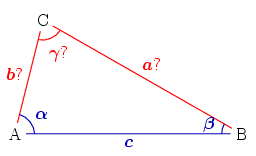
\includegraphics[scale=0.5]{Resolve_triangle_with_c_alpha_beta}
\par\end{center}

The known characteristics are the side c and the angles $\alpha,\beta$.
The third angle $\gamma=180^{\circ}-\alpha-\beta$.

\noindent Two unknown side can be calculated from the law of sines:

\noindent \begin{center}
${\displaystyle a=\frac{c\sin\alpha}{\sin\gamma}}$; ${\displaystyle \quad b=\frac{c\sin\beta}{\sin\gamma}}$. 
\par\end{center}

The procedure for solving an AAS triangle is same as that for an ASA
triangle: First, find the third angle by using the angle sum property
of a triangle, then find the other two sides using the law of sines.


\subsection{SAS Triangle}

\noindent \begin{center}
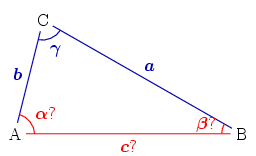
\includegraphics[scale=0.5]{Resolve_triangle_with_a_b_gamma}
\par\end{center}

Here the lengths of sides $a,b$ and the angle $\gamma$ between these
sides are known. The third side can be determined from the law of
cosines:

\noindent \begin{center}
$c=\sqrt{a^{2}+b^{2}-2ab\cos\gamma}$
\par\end{center}

Now we use law of cosines to find the second angle:

\noindent \begin{center}
${\displaystyle \alpha=\cos^{-1}\frac{b^{2}+c^{2}-a^{2}}{2bc}}$
\par\end{center}

Finally, $\beta=180^{\circ}-\alpha-\gamma.$


\subsection{SSS Triangle}

\noindent \begin{center}
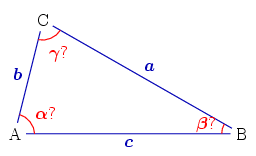
\includegraphics[scale=0.5]{Resolve_triangle_with_a_b_c}
\par\end{center}

Let three side lengths $a,b,c$ be specified. To find the angles $\alpha,\beta$,
the law of cosines can be used:

\noindent \begin{center}
${\displaystyle \alpha=\cos^{-1}\frac{b^{2}+c^{2}-a^{2}}{2bc}}$;${\displaystyle \quad\beta=\cos^{-1}\frac{a^{2}+c^{2}-b^{2}}{2ac}}.$
\par\end{center}

Then angle $\gamma=180^{\circ}-\alpha-\beta$.


\subsection{SSA Triangle}

\noindent \begin{center}
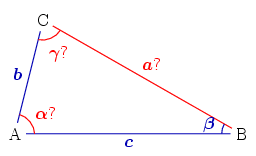
\includegraphics[scale=0.5]{Resolve_triangle_with_b_c_beta}
\par\end{center}

This case is not solvable in all cases; a solution is guaranteed to
be unique only if the side length adjacent to the angle is shorter
than the other side length. Assume that two sides $b$, $c$ and the
angle $\beta$ are known. The equation for the angle $\gamma$ can
be implied from the law of sines:

\noindent \begin{center}
${\displaystyle \sin\gamma=\frac{c\sin\beta}{b}}$
\par\end{center}

We denote further $D=\frac{c\sin\beta}{b}$ (equation's right side).
There are four possible cases:
\begin{enumerate}
\item If $D>1$, no such triangle exists because the side $b$ does not
reach line $BC$. For the same reason a solution does not exist if
the angle $\beta\ge90^{\circ}$ and $b\le c$.
\item If $D=1$, a unique solution exists: $\gamma=90^{\circ}$, i.e., the
triangle is right-angled.
\item If $D<1$, two alternatives are possible.\\
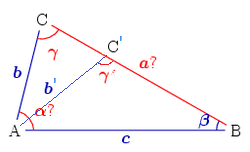
\includegraphics[scale=0.75]{Resolve_triangle_with_b_c_beta_2_solutions}

\begin{enumerate}
\item If $b<c$, the angle $\gamma$ may be acute: $\gamma=\sin^{-1}D$
or obtuse: $\gamma'=180^{\circ}-\gamma$. The picture above shows
the point $C$, the side $b$ and the angle $\gamma$ as the first
solution, and the point $C'$, side $b'$ and the angle $\gamma'$
as the second solution.
\item If $b\ge c$ then $\beta\ge\gamma$ (the larger side corresponds to
a larger angle). Since no triangle can have two obtuse angles, $\gamma$
is acute angle and the solution $\gamma=\sin^{-1}D$ is unique.
\end{enumerate}
\end{enumerate}
Once $\gamma$ is obtained, the third angle $\alpha=180^{\circ}-\beta-\gamma$
.

The third side can then be found from the law of sines:

\noindent \begin{center}
${\displaystyle a=\frac{b\sin\alpha}{\sin\beta}}$
\par\end{center}

\vfill{}



\section{Polar Coordinates}

A point $P$ can be located by rectangular coordinates $\left(x,y\right)$
or polar coordinates $\left(r,\theta\right)$.

The angle $\theta$ is a \emph{directed angle}, that is, it is positive
if it is measured counterclockwise from the initial side to the terminal
side, and negative if it is measured clockwise.

The value $r$ is a \emph{directed distance}, it is positive if the
point $P$ lies on the terminal side of $\theta$ and negative if
$P$ is on the extension of the terminal side.


\subsection{Properties}
\begin{itemize}
\item Every ordered pair of polar coordinates $\left(r,\theta\right)$ locates
a unique point in the plane.
\item However, a point $P$ on the plane may be specified by an infinite
number of ordered pairs $\left(r,\theta\right)$.
\item The pole $O$ may be specified by the ordered pair $\left(0,\theta\right)$
where $\theta\in\mathbb{R}.$
\item Let $P\left(r,\theta\right)$ be a point in the polar plane. Then
$\left(r,\theta+2k\pi\right)$ are also coordinates of the point $P$
for any $k\in\mathbb{Z}$.
\item It can also be shown that $\left(\left(-1\right)^{n}r,\theta+n\pi\right)$
are also coordinates of $P$, where $n\in\mathbb{Z}.$
\end{itemize}

\subsection{Coordinate Transformation}


\subsubsection*{Polar to Rectangular}

\[
\begin{cases}
x=r\cos\theta\\
y=r\sin\theta
\end{cases}
\]



\subsubsection*{Rectangular to Polar}

\[
\begin{cases}
r=\pm\sqrt{x^{2}+y^{2}}\\
\theta=\tan^{-1}\left(y,x\right)
\end{cases}
\]


where $\tan^{-1}\left(y,x\right)$ is the two-argument form of the
arctangent function (see section 3.9).


\section{Special Polar Graphs}


\subsubsection*{Theorem}

A polar graph is:
\begin{enumerate}
\item \textbf{symmetric with respect to the polar axis} if an equivalent
equation is obtained when $\left(r,\theta\right)$ is replaced by
either $\left(r,-\theta\right)$ or $\left(-r,\pi-\theta\right)$.
\item \textbf{symmetric with respect to the $\boldsymbol{\frac{\pi}{2}}$-axis}
if an equivalent equation is obtained when $\left(r,\theta\right)$
is replaced by either $\left(r,\pi-\theta\right)$ or $\left(-r,-\theta\right)$.
\item \textbf{symmetric with respect to the pole} if an equivalent equation
is obtained when $\left(r,\theta\right)$ is replaced by either $\left(-r,\theta\right)$
or $\left(r,\pi+\theta\right)$.
\end{enumerate}

\subsection{Lima�on of Pascal}

A polar equation of the form $r=a+b\cos\theta$ or $r=a+b\cos\theta$
has a polar graph which is called a \emph{lima�on}.

Let $OQ$ be a line joining origin $O$ to any point in $Q$ on a
circle of diameter $b$ passing through $O$. Then the curve is the
locus of all points in $P$ such that $\left|PQ\right|=a$.


\subsubsection*{Types of Lima�ons}
\begin{itemize}
\item Looped lima�on if $0<\left|\frac{a}{b}\right|<1$\\
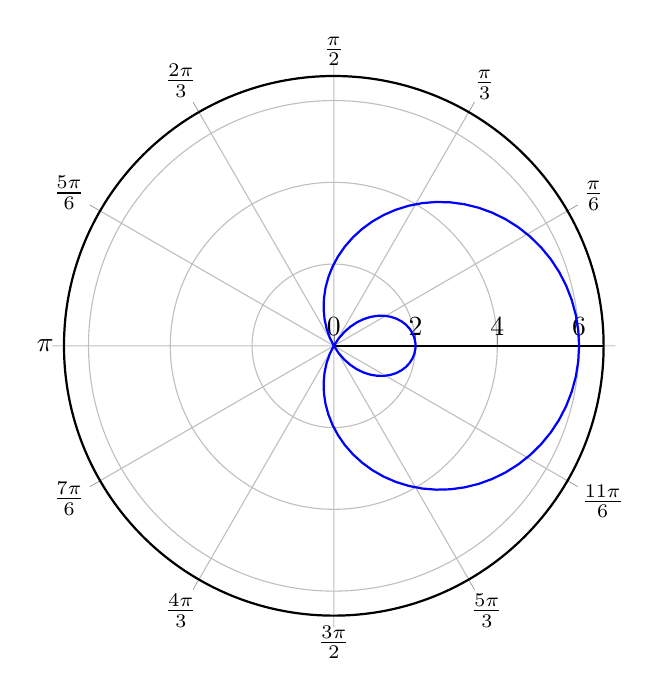
\begin{tikzpicture} \begin{polaraxis}[my style polar] \addplot[color=blue,domain=0:360, samples=100]{2+4*cos(x)}; \end{polaraxis} \end{tikzpicture}
\item Cardioid if $\left|\frac{a}{b}\right|=1$\\
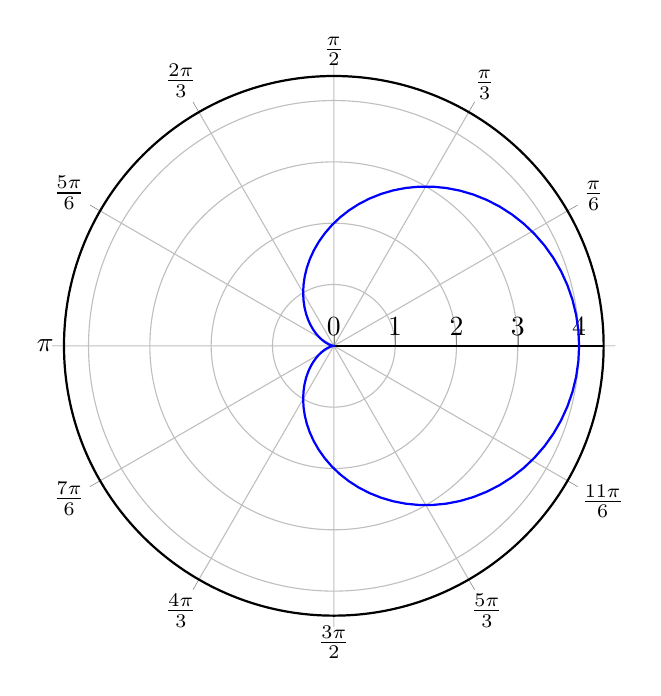
\begin{tikzpicture} \begin{polaraxis}[my style polar] \addplot[color=blue,domain=0:360, samples=100]{2+2*cos(x)}; \end{polaraxis} \end{tikzpicture}
\item Dimpled lima�on if $1<\left|\frac{a}{b}\right|<2$\\
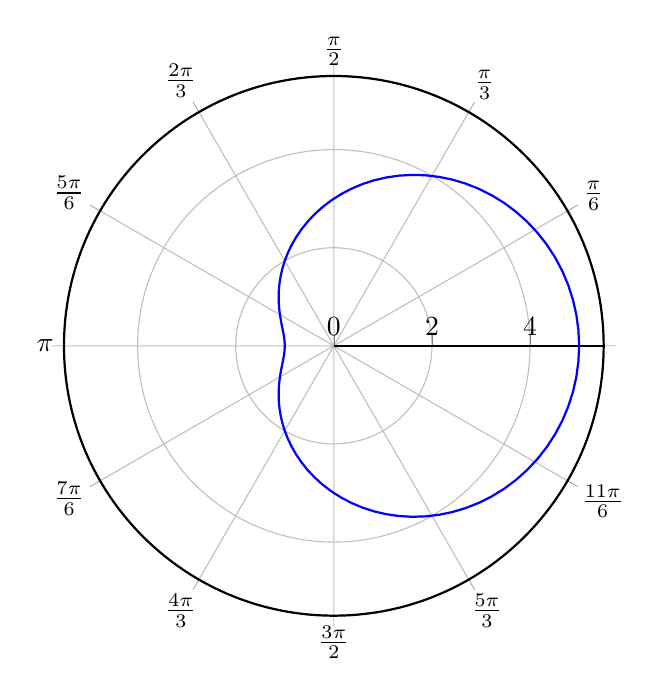
\begin{tikzpicture} \begin{polaraxis}[my style polar] \addplot[color=blue,domain=0:360, samples=100]{3+2*cos(x)}; \end{polaraxis} \end{tikzpicture}
\item Convex lima�on if $\left|\frac{a}{b}\right|\ge2$\\
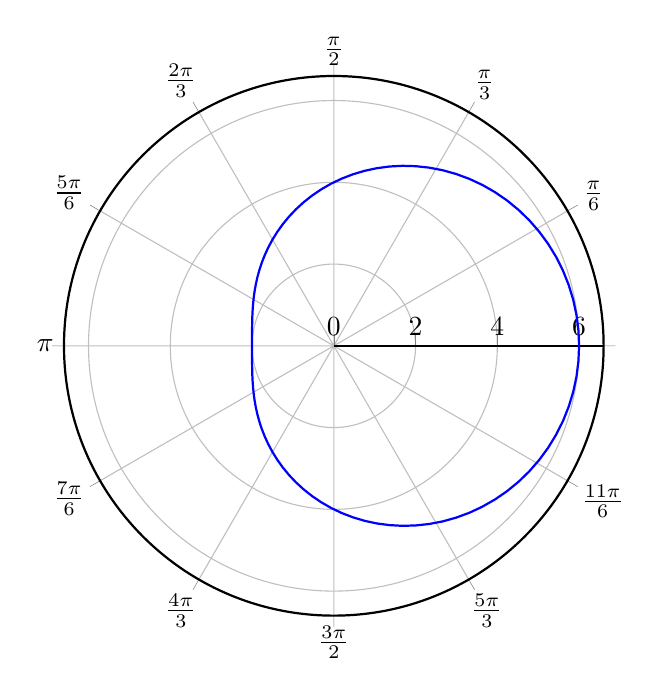
\begin{tikzpicture} \begin{polaraxis}[my style polar] \addplot[color=blue,domain=0:360, samples=100]{4+2*cos(x)}; \end{polaraxis} \end{tikzpicture}
\end{itemize}
\newpage{}


\subsection{Roses}

A rose with $n$ leaves has a polar equation $r=a\cos\left(n\theta\right)$
or $r=a\sin\left(n\theta\right)$ where $a$ is a constant and $n$
is an odd integer.

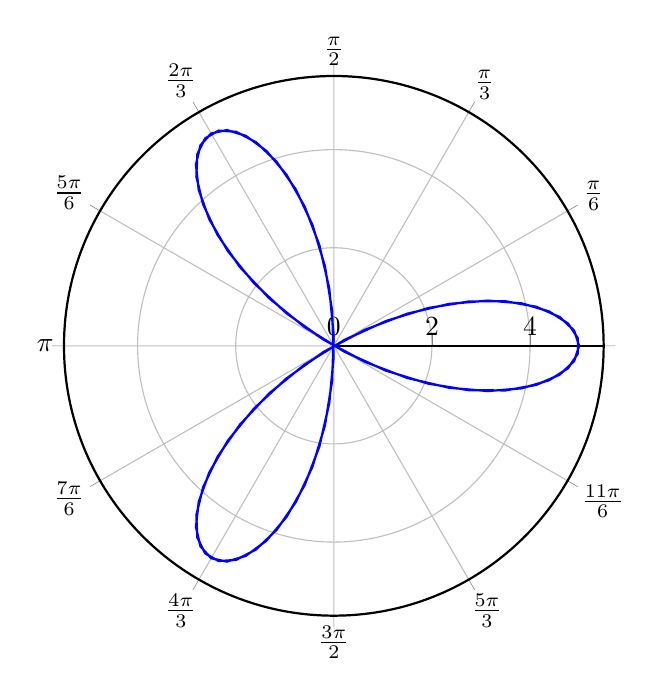
\begin{tikzpicture} \begin{polaraxis}[my style polar] \addplot[color=blue,domain=0:360, samples=100]{5*cos(3*x)}; \end{polaraxis} \end{tikzpicture}

For an even integer $n$, the polar graph of an equation $r=a\cos\left(n\theta\right)$
or $r=a\sin\left(n\theta\right)$ is a rose with $2n$ leaves.

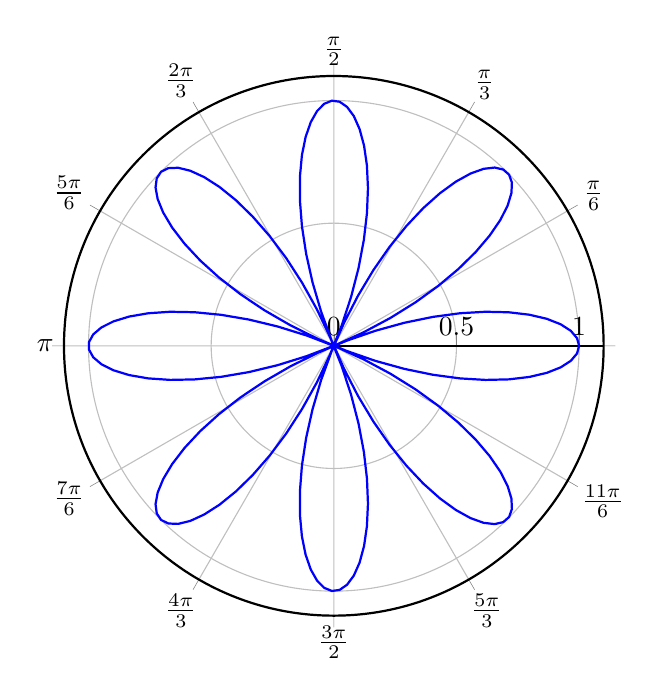
\begin{tikzpicture} \begin{polaraxis}[my style polar] \addplot[color=blue,domain=0:360, samples=200]{cos(4*x)}; \end{polaraxis} \end{tikzpicture}


\subsubsection*{Properties}
\begin{itemize}
\item The length of one leaf in the polar graph of a rose is $\left|a\right|$.
\item If $n$ is odd, then the graph of the polar equation $r=a\cos\left(n\theta\right)$
is symmetric with respect to the polar axis.
\item If $n$ is odd, then the graph of the polar equation $r=a\sin\left(n\theta\right)$
is symmetric with respect to the $\frac{\pi}{2}$-axis.
\item A rose with an even number of leaves is symmetric with respect to
the polar axis, the $\frac{\pi}{2}$-axis, and the pole.
\end{itemize}

\subsection{Spiral of Archimedes}

The polar graph of the polar equation $r=\theta$ where $\theta>0$
is called a \emph{spiral}.

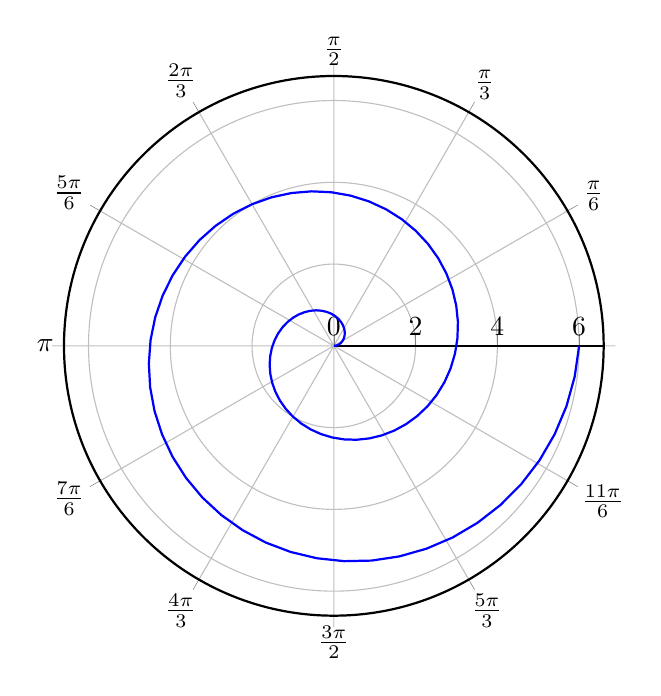
\begin{tikzpicture} \begin{polaraxis}[my style polar] \addplot[color=blue,domain=0:720, samples=100]{x/120}; \end{polaraxis} \end{tikzpicture}


\subsection{Lemniscate of Bernoulli}

A polar equation $r^{2}=a\cos2\theta$ or $r^{2}=a\sin2\theta$ has
a polar graph that is called a \emph{lemniscate}.

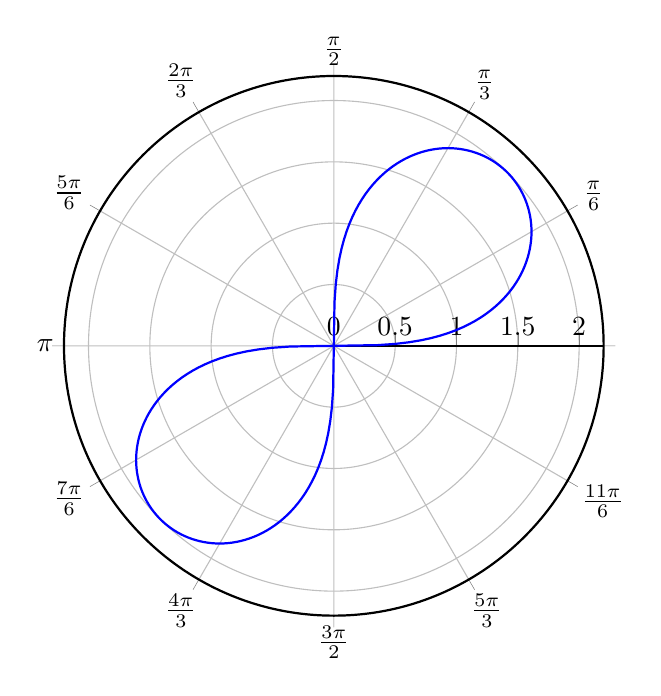
\begin{tikzpicture} \begin{polaraxis}[my style polar] \addplot[color=blue,domain=0:90, samples=100]{2*sqrt(sin(2*x))}; \addplot[color=blue,domain=180:270, samples=100]{2*sqrt(sin(2*x))}; \end{polaraxis} \end{tikzpicture}

\end{multicols*}
\end{document}
